\chapter{結論}
\section{結果總結}
 介紹了Solid Edge 2023新版的優良技術,不管是效率還是人性化的界面都有大大的提升,但並不能說Solid Edge完勝其他3D繪圖軟體,以下將簡單的比較一下Solid Edge與SolidWorks的優劣。\\
 \begin{figure}[hbt!]
\begin{center}
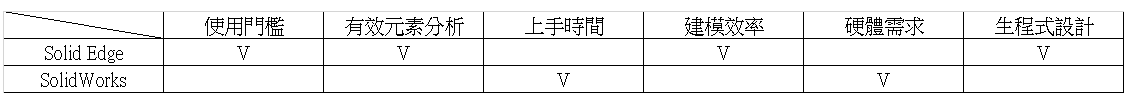
\includegraphics[width=16cm]{對比}
\caption{\Large Solid Edge比較SolidWorks}\label{5.0}
\end{center}
\end{figure}
\\

 由圖\ref{5.0}可知,如果是不熟悉Solid Edge的工程師的話,用起來肯定會認為SolidWorks比較好用,按部就班的程序,能比較好的教導與學習,Solid Edge跟SolidWorks比起來會比較難理解、學習,這就是為什麼目前SolidWorks還是比較廣為人知的原因,但Solid Edge所主打的功能也讓它在繪圖軟體的市場上非常有優勢。\\
 
 不管是多麼熟練的工程師,畫SolidWorks也一定要進到草圖;不管工作效率是多麼高的工程師,設計模型也一定沒有AI來的迅速,而光是同步建模與生成式設計這兩點,就已經足夠讓Solid Edge贏過大多數的繪圖軟體了!\\
 
 
\section{對未來工作的建議}
我認為未來想要開公司的準老闆來說,除了SolidWorks與Autodesk之外,一定還要再把Solid Edge考慮到主要繪圖軟體裡面,只要有一位員工熟悉Solid Edge,勝過對SolidWorks普通了解的2-3位員工。\\

培養Solid Edge繪圖人才,能夠大大的增加公司未來的競爭力,熟用同步建模與生成式設計的人才,光看以上的範例就知道遠勝傳統建模的員工,這投資報酬率遠遠高於讓員工來學習SolidWorks,因為現在會SolidWorks的學生太多了,但會Solid Edge的工程師實在是太少了。\\

剛出社會的新鮮人,如果是不會繪圖軟體的員工的話,就一定要讓他學習Solid Edge,雖然前期一定不會比學SolidWorks來的快,但經過了日經月壘的經驗的話,將熟練度培養起來,肯定不會比學SolidWorks的人來的差,即使培養出Solid Edge的人才數量不多,但只要熟練度夠,Solid Edge團隊肯定會在公司裡發光發熱!\\


\newpage